\chapter{Arhitektura i dizajn sustava}

		\text{Arhitektura aplikacije može se podijeliti na 3 podsustava:}
	\begin{itemize}
		\item 	\text{Web preglednik}
		\item 	\text{Web poslužitelj/Web aplikacija}
		\item 	\text{Baza podataka}		
	\end{itemize}

	\begin{figure}[H]
		\centering
		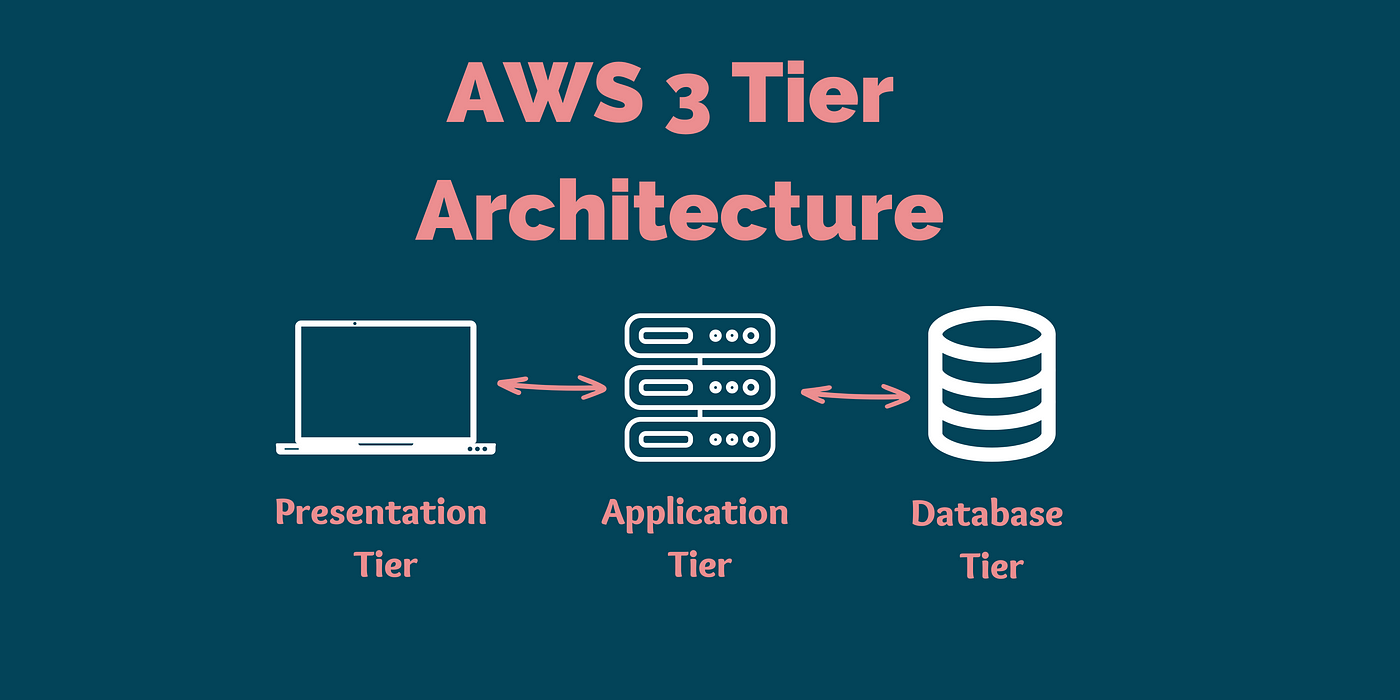
\includegraphics[width=100mm]{slike/arhitektura.png}
		\caption{Arhitektura sustava}
		\label{fig:arhitektura}
	\end{figure}

	\indent{\textit{\underline{Web preglednik(Internetski preglednik)}} je program koji korisniku omogućuje pregled
	web-stranica i multimedijalnih sadržaja vezanih uz njih. Svaki web preglednik je predvoditelj korištenja web aplikacija,
	jer omogućuje korisniku da preko web preglednika šalje zahtjeve web poslužitelju.}

	\indent{\textit{\underline{Web poslužitelj}} je osnova rada web aplikacija. On pokreće cijeli sustav rada aplikacije
	te joj proslijeđuje zahtjeve od korisnika. Osnovna zadaća web poslužitelja je komunikacija korisnika i aplikacije, a ta
	komunikacija se odvija preko HTTP protokola. To je vrsta protokola koja se koristi za prijenos informacija na internetu.}

	\indent{\textit{\underline{Web aplikacija}} je dio web poslužitelja koja služi korisniku za obradu željenih zahtjeva.
	Web aplikacija radi tako da prima zahtjeve i ovisno o zahtjevu pristupa {\textit{\underline{bazi podataka}}} iz koje vuče
	"odgovore" na željene zahtjeve. Te "odgovore" šalje natrag korisniku preko web poslužitelja u obliku HTML dokumenta kojeg
	korisnik vidi u web pregledniku.}

	\indent{Programski jezik kojeg smo odabrali za izradu naše web aplikacije je Python. U sklopu Pythona koristimo Django
	što nije programski jezik, nego Python radni okvir koji služi za izradu web aplikacija. Razvojno okruženje koje koristimo
	je Microsfot Visual Studio Code. Arhitektura sustava temelji se na MVC odnosno MTV konceptu.}

	\indent{Django je modeliran oko MVC okvira, no svoju arhitekturu definira kao MTV (eng. {\textit{Model-Template-View}})
	arhitektura. Komponentu upravitelj (eng. {\textit{Controller}}) zamjenjuje komponentom pogled (eng. {\textit{View}}) te
	komponentu pogled s komponentom predložak (eng. {\textit{Template}}). MTV razdvaja različite dijelove web-stranice: prikaz,
	pristup podatcima i logiku web stranice. Također omogućava neovisnu izgradnju web-stranica, povećava sigurnost sustava te
	pojednostavljuje održavanje sustava.}

	\noindent{MTV sastoji se od:}
	\begin{itemize}
		\item 	\textbf{Model} - definira oblike i odnose podataka u bazama podataka. Model u Django okruženju je klasa napisana
				u programskom jeziku Python. Određuje varijable i metode pridužene određenim tipovima podataka te ima značenje
				tablice u bazi podataka. Model je usko povezan s bazom podataka i pogledom. Od baze podataka model dohvaća tražene
				podatke i prodljeđuje ih pogledu.
		\item 	\textbf{Predložak} - sloj arhitekture MTV - a usko povezan s web-preglednikom. Predložak je HTML stranica s dodanim
				strukturama koje omogućavaju prikaz podataka koji su proslijeđeni od pogleda. Zadaća predloška je sadržaj primljen
				od pogleda organizirati i ugraditi u HTML kod koji će se prikazati u web-pregledniku.
		\item 	\textbf{Pogled} - određuje koji će podatci biti prikazani, odnosno, koji će podatci biti dohvaćeni iz baze podataka
				i prikazani pomoću predloška u web-pregledniku. U Djangu prilikom stvaranja nove web-aplikacije za svaku pojedinu
				aplikaciju stvara se zasebna datoteka pogleda. Pogled ne zna kako su podatci prikazani u web-pregledniku. Posao
				pogleda je dohvatiti tražene podatke i proslijediti ih višem sloju koji će ih prikazati u pregledniku.
	\end{itemize}
	
		

		

				
		\section{Baza podataka}
			
			\textbf{\textit{dio 1. revizije}}\\
			
		\textit{Potrebno je opisati koju vrstu i implementaciju baze podataka ste odabrali, glavne komponente od kojih se sastoji i slično.}
		
			\subsection{Opis tablica}
			

				\textit{Svaku tablicu je potrebno opisati po zadanom predlošku. Lijevo se nalazi točno ime varijable u bazi podataka, u sredini se nalazi tip podataka, a desno se nalazi opis varijable. Svjetlozelenom bojom označite primarni ključ. Svjetlo plavom označite strani ključ}
				
				
				\begin{longtblr}[
					label=none,
					entry=none
					]{
						width = \textwidth,
						colspec={|X[6,l]|X[6, l]|X[20, l]|}, 
						rowhead = 1,
					} %definicija širine tablice, širine stupaca, poravnanje i broja redaka naslova tablice
					\hline \SetCell[c=3]{c}{\textbf{korisnik - ime tablice}}	 \\ \hline[3pt]
					\SetCell{LightGreen}IDKorisnik & INT	&  	Lorem ipsum dolor sit amet, consectetur adipiscing elit, sed do eiusmod  	\\ \hline
					korisnickoIme	& VARCHAR &   	\\ \hline 
					email & VARCHAR &   \\ \hline 
					ime & VARCHAR	&  		\\ \hline 
					\SetCell{LightBlue} primjer	& VARCHAR &   	\\ \hline 
				\end{longtblr}
				
				
			
			\subsection{Dijagram baze podataka}
				\textit{ U ovom potpoglavlju potrebno je umetnuti dijagram baze podataka. Primarni i strani ključevi moraju biti označeni, a tablice povezane. Bazu podataka je potrebno normalizirati. Podsjetite se kolegija "Baze podataka".}
			
			\eject
			
			
		\section{Dijagram razreda}
		
			\textit{Potrebno je priložiti dijagram razreda s pripadajućim opisom. Zbog preglednosti je moguće dijagram razlomiti na više njih, ali moraju biti grupirani prema sličnim razinama apstrakcije i srodnim funkcionalnostima.}\\
			
			\textbf{\textit{dio 1. revizije}}\\
			
			\textit{Prilikom prve predaje projekta, potrebno je priložiti potpuno razrađen dijagram razreda vezan uz \textbf{generičku funkcionalnost} sustava. Ostale funkcionalnosti trebaju biti idejno razrađene u dijagramu sa sljedećim komponentama: nazivi razreda, nazivi metoda i vrste pristupa metodama (npr. javni, zaštićeni), nazivi atributa razreda, veze i odnosi između razreda.}\\
			
			\textbf{\textit{dio 2. revizije}}\\			
			
			\textit{Prilikom druge predaje projekta dijagram razreda i opisi moraju odgovarati stvarnom stanju implementacije}
			
			
			
			\eject
		
		\section{Dijagram stanja}
			
			
			\textbf{\textit{dio 2. revizije}}\\
			
			\textit{Potrebno je priložiti dijagram stanja i opisati ga. Dovoljan je jedan dijagram stanja koji prikazuje \textbf{značajan dio funkcionalnosti} sustava. Na primjer, stanja korisničkog sučelja i tijek korištenja neke ključne funkcionalnosti jesu značajan dio sustava, a registracija i prijava nisu. }
			
			
			\eject 
		
		\section{Dijagram aktivnosti}
			
			\textbf{\textit{dio 2. revizije}}\\
			
			 \textit{Potrebno je priložiti dijagram aktivnosti s pripadajućim opisom. Dijagram aktivnosti treba prikazivati značajan dio sustava.}
			
			\eject
		\section{Dijagram komponenti}
		
			\textbf{\textit{dio 2. revizije}}\\
		
			 \textit{Potrebno je priložiti dijagram komponenti s pripadajućim opisom. Dijagram komponenti treba prikazivati strukturu cijele aplikacije.}